\section{Triple Graph Grammars (TGGs)}

This task mainly deals with specifying bidirectional model-to-text transformations. 
More specifically, it deals with defining a Triple Graph Grammar to transform the tree generated by the parser to  an instance of the ProcessLanguage metamodel and back.


A TGG is basically just a bundle of rules. 
Each rule consists of a source, a target, and a correspondence component.  
Basically, the components consist of object and link variables (just as SDM story patterns). 
The types of the variables in the source, target and correspondence component are defined by the source, the target and correspondence metamodel, respectively.
In our example, the source metamodel is \texttt{MocaTree} and the target metamodel is \texttt{ProcessDefinition}. 
The correspondence metamodel defines the connections between the source and the target metamodel. 
It is specified in the so-called TGG schema. The TGG schema consists of (relevant parts of) the source metamodel, the correspondence metamodel and (relevant parts of) the target metamodel.

You can take a look at TGG schema of our example by double clicking the 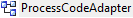
\includegraphics[height=0.3cm]{figures/processCodeAdapterMM.png} icon.


The TGG rules are located in the \texttt{Rules} package.  

If you expand the \texttt{Rules} package and double-click 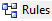
\includegraphics[height=0.3cm]{figures/RulesMM.png}. You see the following rules:
\begin{itemize}
   \item \textbf{RootToSystemRule,} transforms a folder to a \texttt{SystemModule}
   \item \textbf{SubFolderToModuleRule,} transforms a (sub)\texttt{Folder} to a \texttt{Module}
   \item \textbf{FileToTaskRule,} transforms a \texttt{File} to a \texttt{Task}
   \item \textbf{NodeToInvocationRule,} translates the invocations
   \item \textbf{NodeToInvocationRecursiveRule,} translates recursive invocations
   \item \textbf{NodeToInvocationDifferentModuleRule,} translates invocations of tasks contained in a different \texttt{Module}
   \item \textbf{NodeToImportRule,} translates the imports 
\end{itemize}
You can inspect a rule by double clicking on it.


\subsection{Completing the NodeToImportRule}

If you open the \texttt{NodeToImportRule}, you can see that the target and correspondence component are missing. 
Your task is to complete the rule.  


However, before you start, let's take a closer look on how to generate code and execute the transformation. 
Therefore, \textbf{(1)} export the project, \textbf{(2)} go back to Eclipse, \textbf{(3)} select the \texttt{ProcessLanguage} project and press F5. The code generation process starts. 
After the process has finished, open the file \texttt{org.moflon.moca.MocaMain.java} located in the \texttt{ProcessCodeAdapter} Project. 
This class implements the workflow described in Section \ref{sec: The workflow for compiling and validating instances}. 
It takes the instance from \texttt{ProcessCodeAdapter/instances/in} performs the text to model transformation and immediately afterwards the model to text transformation. The result is written to \texttt{ProcessCodeAdapter/instances/out}. 
Run the file and compare the input and outputs (note: you may have to refresh the instances folder). 
As expected the import statements are missing. 


Now complete the \texttt{NodeToImportRule} rule so that the import statements are translated.
For specifying the rule it might be helpful to know the structure of the tree generated by the parser. An instance can be found at \texttt{ProcessCodeAdapter/instances/tree}.

\subsection{TGGs in Action}
Since we have a working bidirectional model to text transformation, it is time to see it in action.
As you can imagine, it does not make sense to transform the same instance forward and backward without modifications. Therefore, specify a method using SDMs that automatically adds the missing imports.   
Therefore, create a new method \texttt{checkImports} for the class SystemModule and specify the SDM. 
 
\textbf{Test:}\\
To test your SDM export it and generate code.
Run the generated method by calling it below the \texttt{//validation} comment in the \texttt{MocaMain.java} and see if the missing import statements are added. 








